% !TEX root= ../main.tex
\documentclass[main.tex]{subfiles}

\begin{document}
\section{PŘESTUP TEPLA V TEKUTÝCH KOVECH}

\lipsum[2]
\begin{gather}
    \text{Nu}=0.25+6.2x+(0.032x-0.007)\cdot \text{Pe}^{0.8-0.024x}\\
    \alpha=\frac{\lambda}{L}\cdot\left[0.25+6.2x+(0.032x-0.007)\cdot \left(\frac{L\cdot v}{a}\right)^{0.8-0.024x}\right]
\end{gather}

\begin{figure}[hbt]
    \centering
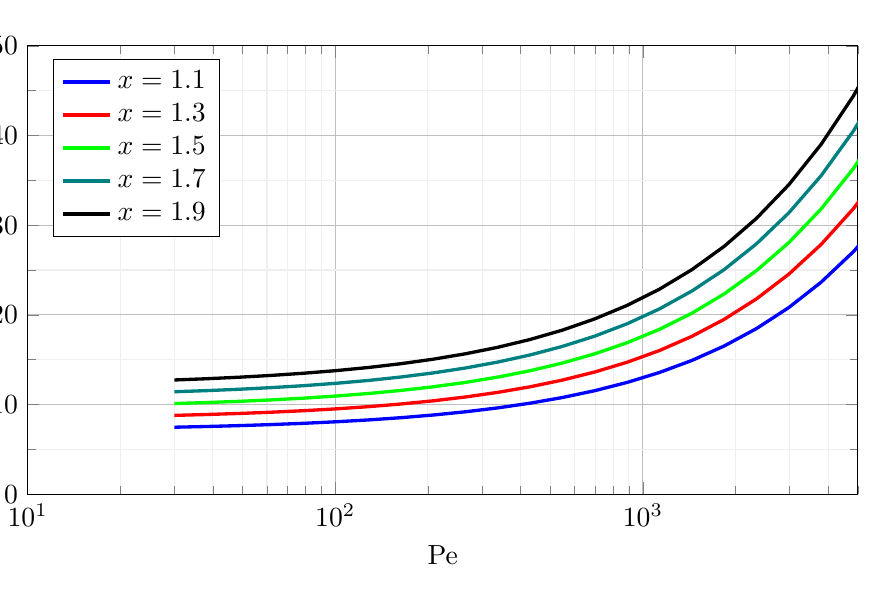
\begin{tikzpicture}[trim left]
        \begin{axis}[
            xmin = 10, xmax = 5000,
            ymin = 0, ymax = 50,
            xmode=log,
            ytick distance = 10,
            grid = both,
            minor tick num = 1,
            major grid style = {lightgray},
            minor grid style = {lightgray!25},
            legend cell align = {left},
            legend pos = north west,
            xlabel = Pe,
            ylabel = Nu,
            width = \textwidth,
            height = 0.6\textwidth,
            every axis plot/.append style={very thick},
        ]
            \addplot[blue,domain = 30:10000]{0.25+6.2*1.1+(0.032*1.1-0.007)*x^(0.8-0.024*1.1)};
            \addplot[red,domain = 30:10000]{0.25+6.2*1.3+(0.032*1.3-0.007)*x^(0.8-0.024*1.3)};
            \addplot[green,domain = 30:10000]{0.25+6.2*1.5+(0.032*1.5-0.007)*x^(0.8-0.024*1.5)};
            \addplot[teal,domain = 30:10000]{0.25+6.2*1.7+(0.032*1.7-0.007)*x^(0.8-0.024*1.7)};
            \addplot[black,domain = 30:10000]{0.25+6.2*1.9+(0.032*1.9-0.007)*x^(0.8-0.024*1.9)};
            \legend{
                \(x=1.1\),
                \(x=1.3\),
                \(x=1.5\),
                \(x=1.7\),
                \(x=1.9\),
             }
        \end{axis}
    \end{tikzpicture}
    \caption{Podélné obtékání trubek.}
\end{figure}
\clearpage

\begin{equation}
    \text{Nu}=\Delta^{0.3}\cdot(x_1+x_2\cdot\text{Pe}^{x_3})
\end{equation}
Kde:
\begin{itemize}
\setlength{\parskip}{0pt}
    \item \(x_1=4.75\)
    \item \(x_2=0.0175\)
    \item \(x_3=0.8\)
    \item \(\Delta=\frac{D}{d}=1\div7\)
\end{itemize}
\begin{gather}
    \text{Nu}=\Delta^{0.3}\cdot(4.75+0.0175\cdot\text{Pe}^{0.8})\\
    \alpha=\frac{\lambda}{L}\cdot\left\{\Delta^{0.3}\cdot\left[4.75+0.0175\cdot\left(\frac{L\cdot v}{a}\right)^{0.8}\right]\right\}
\end{gather}


\begin{figure}[hbt]
    \centering
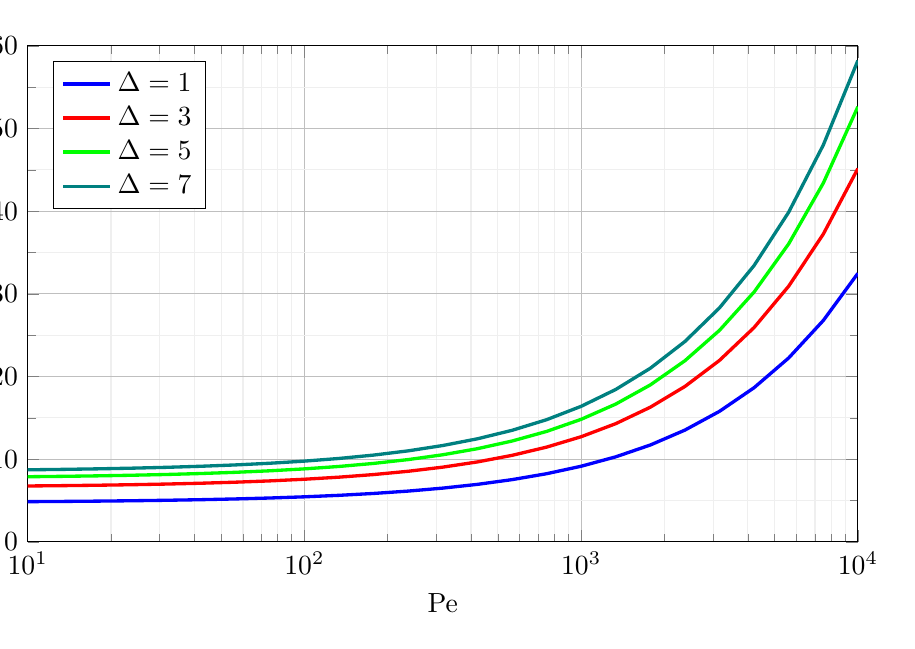
\begin{tikzpicture}[trim left]
        \begin{axis}[
            xmin = 10, xmax = 10000,
            ymin = 0, ymax = 60,
            xmode=log,
            ytick distance = 10,
            grid = both,
            minor tick num = 1,
            major grid style = {lightgray},
            minor grid style = {lightgray!25},
            legend cell align = {left},
            legend pos = north west,
            xlabel = Pe=Re\(\cdot\)Pr,
            ylabel = Nu,
            width = \textwidth,
            height = 0.65\textwidth,
        ]
            \addplot[blue,very thick,domain = 10:10000]{1^(0.3)*(4.75+0.0175*x^(0.8))};
            \addplot[red,very thick,domain = 10:10000]{3^(0.3)*(4.75+0.0175*x^(0.8))};
            \addplot[green,very thick,domain = 10:10000]{5^(0.3)*(4.75+0.0175*x^(0.8))};
            \addplot[teal,very thick,domain = 10:10000]{7^(0.3)*(4.75+0.0175*x^(0.8))};
            \legend{
                \(\Delta=1\),
                \(\Delta=3\),
                \(\Delta=5\),
                \(\Delta=7\),}
        \end{axis}
    \end{tikzpicture}
    \caption{Predikce přestupu tepla v mezikruhovém kanálu.}
\end{figure}
\end{document}
